% oneside to ensure no unnecessary blank pages are inserted and margins are equal across both odd and even pages.
\documentclass[oneside, whitelogo]{tudelft-report}

\usepackage{wrapfig}
\begin{document}
	
	%% Use Roman numerals for the page numbers of the title pages and table of
	%% contents.
	\frontmatter
	
	% Title and subtitle color can be configured by entering a colour as parameter for the subtitle command. 
	\title{Pantzerfaust\\DNav}
	\subtitle[tudelft-white]{Final Product Report}
	\author[tudelft-white]{
		W.\ Smit\\
		J.\ van der Krieken\\
		C.\ Athmer\\
		F.\ Elghlan\\
		C.\ Bilstra\\
	}
	\affiliation{Delft University of Technology} 
	\coverimage{cover.jpg}
	\titleoffsetx{1cm}
	\titleoffsety{6.5cm}
	\afiloffsetx{1cm} 
	\afiloffsety{18cm} 
	
	\makecover
	
	%% Include an optional title page.
	\begin{titlepage}
	
	\begin{center}
		
		%% Insert the TU Delft logo at the bottom of the page.
		\begin{tikzpicture}[remember picture,overlay]
		\node at (current page.south)[anchor=south,inner sep=0pt]{
			
\includegraphics{cover/logo}
		};
		\end{tikzpicture}
		
		%% Print the title in cyan.
		{\makeatletter
			\tudtitlefamily\color{tudelft-cyan}\fontsize{64}{94}\selectfont\@title
			%\largetitlestyle\color{tudelft-cyan}\Huge\@title
			\makeatother}
		
		%% Print the optional subtitle in black.
		{\makeatletter
			\ifx\@subtitle\undefined\else
			\bigskip
			{\tudsffamily\color{tudelft-cyan}\fontsize{22}{32}\selectfont\@subtitle}    
			%\titlefont\titleshape\LARGE\@subtitle
			\fi
			\makeatother}
		
		\bigskip
		\bigskip
		
		by
		%door
		
		\bigskip
		\bigskip
		
		%% Print the name of the author.
		{\makeatletter
			%\largetitlefont\Large\bfseries\@author
			\tudtitlefamily\color{tudelft-black}\fontsize{26}{26}\selectfont\@author
			\makeatother}
		
		\bigskip
		\bigskip
		\bigskip
		
		\begin{tabular}{llll}
			\multicolumn{4}{l}{Student numbers:}\\
			
			Wouter Smit & 4401409 & Faris Elghlan & 4341538\\
			Justin van der Krieken & 4357116 & Cas Bilstra & 4381084\\
			Casper Athmer & 4329066 &\\
			
			\\
			\multicolumn{2}{l}{Project duration:} & \multicolumn{2}{l}{April 18, 2016 -- June 23, 2016} \\
			\multicolumn{2}{l}{Context coordinator:} & \multicolumn{2}{l}{Thomas Abeel} \\ 
			\multicolumn{2}{l}{Customer representative:} & \multicolumn{2}{l}{Thomas Abeel} \\ 
			\\
			\multicolumn{2}{l}{Teaching Assistants:} & \multicolumn{2}{l}{Sjoerd Huisman}\\
			\multicolumn{2}{l}{} & \multicolumn{2}{l}{Jasper Linthorst}\\
			\\
			\multicolumn{2}{l}{Software Teaching Assistant:} & \multicolumn{2}{l}{Jim Hommes}\\
		\end{tabular}
		
		%% Only include the following lines if confidentiality is applicable.
		\bigskip
		\bigskip
		\emph{}
		%\emph{}
		
		\bigskip
		\bigskip
		
	\end{center}
	
\end{titlepage}
	
	\tableofcontents
	
	%% Chapters are separated into files. 
	
	%% Use Arabic numerals for the page numbers of the chapters.
	\mainmatter
	
	\chapter{Introduction}
\par
Tuberculosis is a big problem in modern society. It’s a deadly disease (if untreated, the disease kills about half of those infected) and about one third of the world population is infected with it \citep{whoTB}. Curing this disease takes at least six months with the current medicines and possibly up to three years in which six variants of antibiotics have to be taken\citep{p1TB}.
\par
Drug-resistant tuberculosis is becoming an increasingly difficult problem. Research is being done in order to make new vaccines, drugs and diagnostics to improve the ability to cure this disease. One of the institutes performing this research is the Broad Institute, an institute for biomedical science, which is being run by MIT and Harvard. To do this research efficiently, an application to compare and visualize multiple DNA sequences (genomes) is needed. Last year an attempt was made by students from the Delft University of Technology, but the applications they created did not suffice. The main problems were that programs were not scalable (they could only load a small dataset of genomes) and missed semantic zooming. This year the development project is repeated. This report describes the development of such an application, which can help biologists explore Tuberculosis genomes.
\par
The goal for this application is to create a tool for interactive visualization of DNA sequence graphs to enable exploratory data analysis. The application must comply with the following requirements:
\begin{itemize}
	\item The visualization must be interactive (i.e. the user should be able to easily navigate the visualization).
	\item Semantic zooming. The customer expects to be able to zoom in onto the visualization. As the visualization is more zoomed in, more information should become visible.
	\item Integration between phylogeny (i.e. ancestral history of genomes) and the genomes. Usually represented as a tree. Such tree could be used as navigation device.
	\item Metadata about genomes and annotations of parts of (the reference) genome should be integrated. Ideally these should be easily accessible (e.g. searchable).
\end{itemize}

Lastly, the customer would like to be able to detect a phenomenon called convergent evolution. This occurs when two two separate branches of the evolution of the genome separately mutated in the same way. This indicates that this mutation is likely to happen evolutionary, regardless of previous mutations of a genome.

	\input{chapters/OverviewOfThefinalProduct}
	\chapter{Reflection on the product and development process (SEM)}
This section evaluates the development process of the product and the technical aspects of the product. The evaluation of the development process includes evaluating the dynamics in the group, the use of sprints and the documentation. Evaluating the technical aspects of the project focuses on the quality of the code. 

\section{Development process}
\par
The dynamics in the group were good. The communication in the group went through different channels, including e-mail, WhatsApp, Slack, GitHub, and face-to-face. In retrospect, it would have been better to have less channels of communication, because checking all aforementioned channels is cumbersome. However, during this project the high number of communication channels did not cause problems. 
\par
During this project, a new sprint planning was made weekly. This was not ideal, because a sprint of a week is short, and there have been big tasks which take longer than a week, which are therefore hard to put in a sprint planning. 
\par
The sprint plannings that have been made also tended to include too much work for a week. Often, the development of new features took longer than was accounted for in the spring planning, which meant not all tasks on the planning were done. For future projects, it’s important to better estimate the time it costs to develop new features.
\par
The formal documentation during this project included an Architecture Design, the weekly sprint planning and sprint retrospective. This documentation has not been used by any member of the group during the development phase. A useful form of documentation were the issues on GitHub. These were used extensively, and showed a nice overview of tasks to be done. 

\section{Product evaluation}
\par
The code for the application has been split in modules. A big advantage of this is that a module can be taken out and replaced with another module, without changing the rest of the code. The use of modules brought challenges with it (e.g. the visibility of classes), but is a nice way to separate code. 
\par
An important principle which has been used a lot, is the use of interfaces. The model classes have all been implemented using an interface, which makes it more reusable. 
A part of the program which is not as reusable, is the GUI part. Some of the classes in this module have become large, which is inherent to using JavaFX\footnote{http://docs.oracle.com/javase/8/javafx/get-started-tutorial/jfx-overview.htm}. Another reason that this happened, was the fact that the client demanded many new features every week. There is a constant tradeoff to be made between quality of code and the quality of the program (in terms of features). During this project the latter was often preferred.
	
\chapter{Description of the developed functionalities}
This chapter will give a description of the functionalities that are developed for our application. The requirements mentioned in the introduction are used to reflect on the functionalities.
\section{Semantic zooming}
\begin{wrapfigure}{r}{0.2\textwidth}
	\centering
	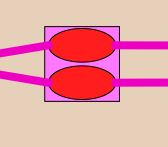
\includegraphics{images/mutation.jpg}
	\caption{\label{fig:bubble}A mutation bubble}
\end{wrapfigure}
Semantic zooming should be provided to the customer which initially shows the entire graph, and on which the user can zoom in to see more details. This is implemented by making bubbles, which collapse nodes together, and showing these at a high-level view. When zooming in (which happens stepless), the bubbles are expanded and more details of the graph are shown. By creating bubbles, large amounts of genomes can be visualized. When nodes in the graph (which represent base sequences) are big enough they become visible. Figure X+1 shows an example of a bubble (the purple square), containing two nodes, which has been expanded. 

\section{Phylogenetic tree}

\begin{wrapfigure}{l}{5cm}
	\centering
	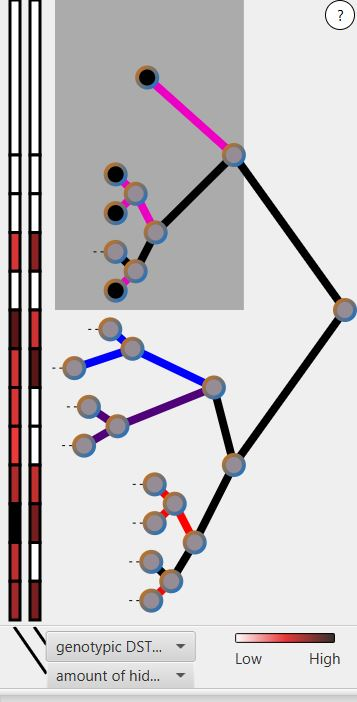
\includegraphics[width=0.3\textwidth]{images/tree.jpg}
	\caption{\label{fig:tree}The phylogenetic\\tree}
\end{wrapfigure}

The phylogenetic tree can be used to visualize a subset of the genomes. The tree in the application can be zoomed in on, because not every leaf node can be shown on the screen when the dataset is big. By zooming in, nodes on a deeper level become visible. 
\par
There exist lineages in the phylogeny, which is a grouping of genomes. These lineages have a specific colour which is shown on the edges between nodes in the tree. 
\par
On the left of the tree is a heatmap which can be used to show the density of properties of the tree (e.g. the number of leaf nodes in a certain branch). 
\par
Nodes can be dragged from the phylogenetic tree to the main graph area and all genomes contained in the leaves of the selected tree are then drawn on the screen. When dragged to the main area a popup will appear asking if the genomes should be added to the existing graph, if a new graph has to be created, or if the specific nodes have to be removed from the current visualization. 
\par
Because the application builds on the idea that the comparison of two graphs can be useful, two graphs can be drawn on the main screen. Nodes in the tree have colouring to indicate in which graph(s) they are present. There is a legend present for all visuals in the tree. 
Figure X+2 shows an example of the phylogenetic tree, with one heatmap containing the amount of hidden nodes in a branch and the other heatmap containing the amount of genotype DST:XDR in a branch.
\section{The main area}
The main area is the part where the graph is drawn. As mentioned before, there can be a graph on the top half and a graph on the bottom half (see figure X). It is also possible to show only one graph. Loading is performed with simple dragging and dropping from the phylogenetic tree. When a graph is loaded, the user sees different rectangles, ellipses, and colours. These represent different types of bubbles, which are explained in the legend. 
\section{Searching}
On the main screen a searching pane is available. A search can be performed based on metadata about the genomes. Multiple genomes that resulted from a search can be selected and dragged to the main graph. This works the same as dragging and dropping from the phylogenetic tree.
\section{Loading}
When the application is started a file loader appears wherein the files to be loaded can be selected. The application supports the .gfa file-format for the graph, the .nwk file-format for the phylogenetic tree, the .gff file-format for the annotations and the .xlsx file-format for the metadata. 
\section{Settings}
There is a settings menu, where the user can select which bubbling algorithms it wants to use (if any). There are five options to choose from, which are explained in the application.
	\chapter{Evaluation of the functional modules and the product in its entirety, including the failure analysis}
To evaluate the functional modules and the product in its entirety, the feedback given by the client about the program is used. The program is made for the client which means that their feedback is most valuable in evaluating the program. The evaluation of the developers is also used for evaluating the program, because the developers know in which areas the program can improve. 

\section{Program evaluation}
Overall the application that is built is good. It meets the wishes of the client and has an extensive list of features. There are issues in the application which have not been solved. These are discussed below.
\subsection{Vertical spacing}
The fact that the client didn’t want vertical scrolling (i.e. all nodes in the vertical spacing are shown on the screen), caused nodes to be barely visible in locations with many branches. One way to solve this would be to add the ability to also zoom vertically, but this was something which was not desirable for the client at this time. Another option would be to use the vertical space more efficiently and to make the nodes smaller.

\subsection{Usability of the program for biologists}
In terms of speed the program has an outstanding performance, which makes it usable. However, the program has a lot of features, which can be overwhelming for a user.The program needs guidelines for a user to be able to use it. 
Another issue with usability relates to the problem of vertical spacing. Because of this problem, more complicated structures in the graph can be not be explored. 
A big issue for the biologists was finding convergent evolution, and our program can still improve in this area. There is some visual help in finding convergent evolution with the phylogenetic bubbles, but it’s open to improvement.  Highlighting convergent evolution in the graph would be a huge improvement. 


	
%	\input{chapters/ProgramOfRequirements}
	
	\bibliographystyle{apalike}
	\bibliography{report}
	
	%% Use letters for the chapter numbers of the appendices.
	\appendix
	%\input{appendices/appendices}
	%\addcontentsline{toc}{chapter}{Appendices}
	
	
	
	
	% All references should be in the bibliography, even when not cited in text.
	\nocite{*}
	
\end{document}